\documentclass{beamer}

%%%%%%%%%%%%%Solarized Theme%%%%%%%%%%%%%%%
\usecolortheme[dark,accent=cyan]{solarized}
\beamertemplatenavigationsymbolsempty

%%%%%Packages%%%%%
\usepackage{graphicx}
\graphicspath{ {static/} }

\usepackage{hyperref}
\usepackage{colortbl, xcolor}
\usepackage{booktabs}
\usepackage{subcaption}

\usepackage{tikz}
\usepackage{standalone}
\usetikzlibrary{decorations.pathmorphing}
\usetikzlibrary{fit}                    
\usetikzlibrary{backgrounds}
\usetikzlibrary{calc}

\usepackage{amsmath}
\usepackage{amsthm}
\usepackage{amssymb}

\setbeamertemplate{blocks}[default]

%%%%%%Title%%%%%%%%
\title{Optimisation of short memory strategies in the Iterated Prisoners Dilemma}
\author{Nikoleta E. Glynatsi}
\date{\tiny{Supervised by:} \\ \small{Dr. Vincent \textsc{Knight} \hspace{1cm}  Dr. Jonathan \textsc{Gillard} }}
\institute[]
{
\begin{center}
    
\includegraphics[width=.20\textwidth]{cardiff_uni_logo.jpg}
\end{center}
}

\begin{document}

\maketitle  

\begin{frame}
  \Huge
    \[
    \begin{bmatrix}
      (3,3) & (0,5)  \\
      (5,0) & (1,1)
    \end{bmatrix}
    \]
  \pause
  \centering
    \Large
      \vfill
      \( (R, P, S, T) = (3, 1, 0, 5) \) 
\end{frame}

\begin{frame}
    \begin{center}
        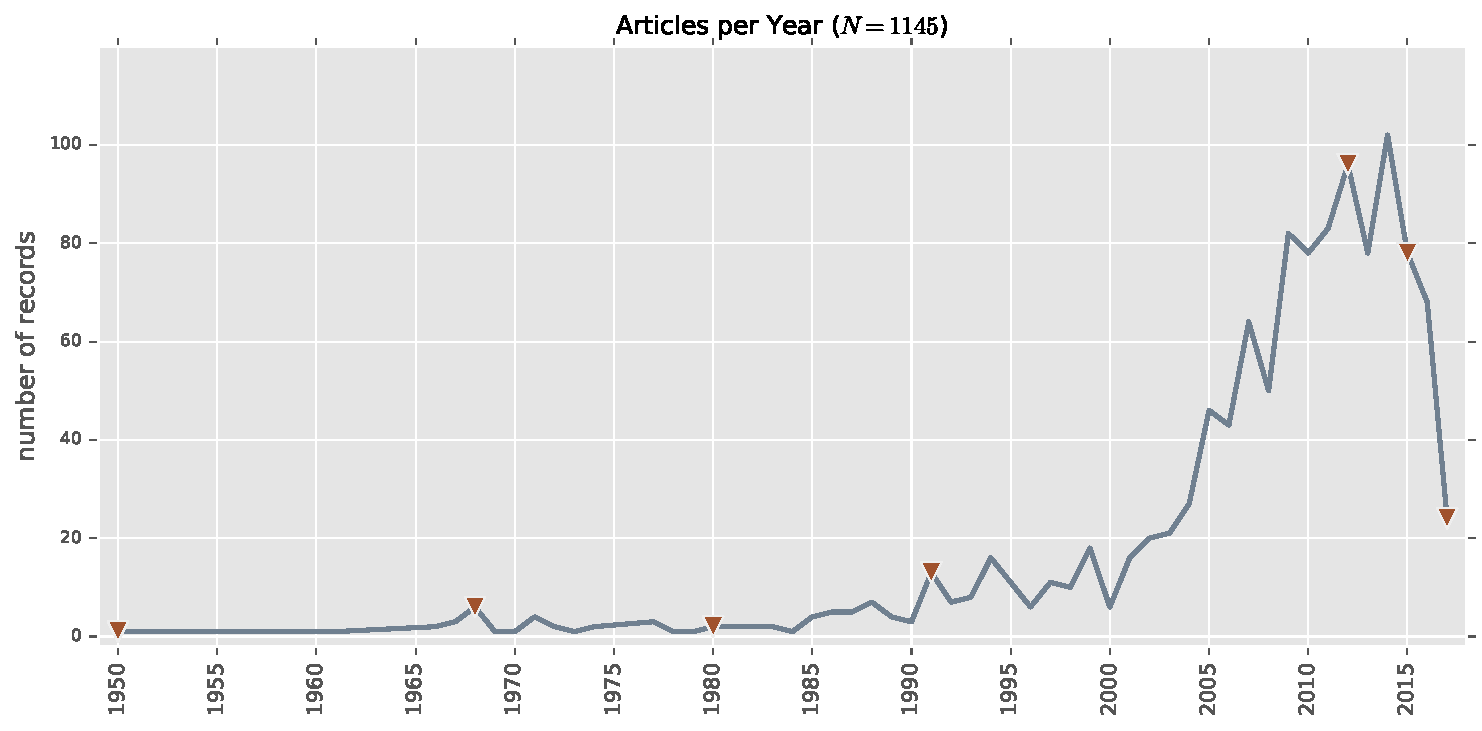
\includegraphics[width=\textwidth, height=0.5\textwidth]{timeline.pdf}
    \end{center}
\end{frame}

\begin{frame}
  \centering
  \includestandalone[width=0.5\textwidth]{memory_one_chain}

  \vfill
  \large
  \( p = (p_1, p_2, p_3, p_4) \in\mathbb{R}_{[0,1]}^{4} \)
\end{frame}


\begin{frame}
    \begin{center}
       \begin{itemize}
        \item  \textit{Christopher Lee, Marc Harper, and Dashiell Fryer.}
               The art of war: Beyond memory-one strategies in population games. 2015.
        \end{itemize}
    \end{center}
\end{frame}

\begin{frame}
    \begin{center}
        \Large How good are memory one strategies ?
    \end{center}
\end{frame}

\begin{frame}
  \centering
  \includestandalone[width=0.6\textwidth]{states}
\end{frame}

\begin{frame}
    \begin{center}
    \small{
           M = \(\begin{bmatrix}
           p_{1} q_{1}& p_{1} (- q_{1} + 1) & q_{1} (- p_{1} + 1) & (- p_{1} + 1) (- q_{1} + 1)
           \\
           p_{2} q_{3} & p_{2} (- q_{3} + 1) & q_{3} (- p_{2} + 1) & (- p_{2} + 1) (- q_{3} + 1)
           \\
           p_{3} q_{2} & p_{3} (- q_{2} + 1) & q_{2} (- p_{3} + 1) & (- p_{3} + 1) (- q_{2} + 1)
           \\
           p_{4} q_{4} & p_{4} (- q_{4} + 1) & q_{4} (- p_{4} + 1) & (- p_{4} + 1) (- q_{4} + 1)\end{bmatrix}\)
           }
    \end{center}
\end{frame}

\begin{frame}
\centering
\huge
\( \max_p u_q(p)\text{ such that }p\in\mathbb{R}_{[0,1]}^{4}\)
\end{frame}

\begin{frame}
    \begin{center}
    \begin{lemma}
     \[ u_q(p) = \frac{\frac{1}{2} p Q  p^T + c^T  p + a} 
    {\frac{1}{2} p \bar{Q} p^T + \bar{c}^T p + \bar{a}}\]

    \begin{itemize}
      \item \(Q, \bar{Q} \in\mathbb{R}^{4 \times 4}\)
      \item \(c, \bar{c}\in\mathbb{R}^{4 \times 1}\) 
      \item \(a, \bar{a}\in\mathbb{R}\)  
   \end{itemize}
    \end{lemma}
    \end{center}
\end{frame}

\begin{frame}
\centering
\huge
\( \max_p u_q(p)\text{ such that }p\in\mathbb{R}_{[0,1]}^{4}\)
\pause
\vfill
\Large
subject to \( p_1 = p_2 = p_3 = p_4 =p\)
\end{frame}

\begin{frame}
\begin{lemma}
\[ u_q(p)  =  \frac{n_2p^2 + n_1p + n_0 } {d_1p + d_0} \]

\begin{itemize}
    \item \( n_{2} = - (q_{1} - q_{2} - 2 q_{3} + 2 q_{4})\)
    \item \( n_{1} = - q_{1} + 2 q_{2} + 5 q_{3} - 7 q_{4} - 1 \)
    \item \( n_{0} =   q_{2} - 5q_{4} - 1\)
    \item \( d_{1} =   q_{1} - q_{2} - q_{3} + q_{4}\)
    \item \( d_{0} =   q_{2} - q_{4} -1\)
\end{itemize}
\end{lemma}
\end{frame}

\begin{frame}
  \centering
  \Large \[ q = \left(1, 1, 0, \frac{2}{3}\right) \]
  \includegraphics[width=0.6\linewidth]{rnd/"1*0000, 1*0000, 0*0000, 0*6667".pdf}
  \pause
  \small
      \begin{equation*} u_q(p) = \frac{-\frac{4p^2}{3} + \frac{14p}{3} - \frac{10}{3}}
                   {\frac{2p}{3} - \frac{2}{3}} \onslide<3->{= -2p + 5}
    \end{equation*} 
\end{frame}

\begin{frame}
  \centering
  \Large \[ q=\left(1, 0, 1, \frac{1}{3}\right) \]
  \includegraphics[width=0.6\linewidth]{rnd/"1*0000, 0*0000, 1*0000, 0*3333".pdf}
  \pause
  \small
    \begin{equation*} u_q(p) = \frac{\frac{p^2}{3} + \frac{8p}{3} - \frac{10}{3}}
                   {\frac{p}{3} - \frac{4}{3}} \onslide<3->{= p + 2}
    \end{equation*} 
\end{frame}

\begin{frame}
   \centering
   \Large \[ q=\left(\frac{2}{3}, 0, \frac{2}{3}, \frac{1}{3}\right) \]
   \includegraphics[width=0.6\linewidth]{rnd/"0*6667, 0*0000, 0*6667, 0*3333".pdf}
   \pause
   \small
    \begin{equation*} u_q(p) = \frac{\frac{2p}{3} - \frac{8}{3}}
                   {\frac{p}{3} - \frac{4}{3}} \onslide<3->{= 2}
    \end{equation*} 
 \end{frame}

\begin{frame}
  \centering
  \Large \[ q=\left(\frac{2}{3}, \frac{1}{3}, \frac{1}{3}, 0\right) \]
  \includegraphics[width=0.6\linewidth]{rnd/"0*6667, 0*3333, 0*3333, 0*0000".pdf}
   \pause
   \small
    \begin{equation*} u_q(p) = \frac{\frac{p^2}{3} - \frac{2p}{3} - \frac{2}{3}}
                   {- \frac{2}{3}} \onslide<3->{= -\frac{p^2}{2} + p + 1}
    \end{equation*} 
\end{frame}


\begin{frame}
\centering
\footnotesize
\begin{lemma}[Indifferent]\label{lemma:constant} 
\( -q_1 + q_2 + 2q_3 - 2q_4 = 0 \) and  \( (q_2 - q_4 - 1)(q_1 - 2q_2 - 5q_3 + 7q_4 + 1) -(q_2 - 5q_4 - 1)(q_1 - q_2 - q_3 + q_4) = 0 .\)
\end{lemma}

\centering
\begin{proof} 
\begin{align*}
u_q(p) = \frac{n_2p^2 + n_1p + n_0 } {d_1p + d_0} & = a_0 \\
n_2p^2 + n_1p + n_0 & = a_0d_1p + a_0d_0 
\end{align*}

\[\begin{cases}
          n_2  = 0\\
          n_1d_0 = d_1n_0
  \end{cases}\]

\end{proof}


\end{frame}

\begin{frame}
\centering
\footnotesize
\begin{lemma}[Linear]\label{lemma:linear}
\((q_{1} 
q_{4} - q_{2} q_{3} + q_{3} - q_{4}) (4 q_{1} - 3 q_{2} - 4 q_{3} 
+ 3 q_{4} - 1) = 0\)
\end{lemma}

\begin{proof} 
\begin{align*}
u_q(p) & = \frac{n_2p^2 + n_1p + n_0 } {d_1p + d_0} = a_1p + a_0 \\
n_2p^2 + n_1p + n_0 & = a_1d_1p^2 + (d_1a_0 + a_1d_0)p + a_0d_0 
\end{align*}
\[\begin{cases}
          n_2 = d_1a_1\\
          n_1d_0 = d_1n_0 + a_1 d_0
  \end{cases}\]
\end{proof}
\end{frame}

\begin{frame}
\centering
\footnotesize
\begin{lemma}[Quadratic]\label{lemma:quadratic}
\((q_{1} - q_{2} - q_{3} + q_{4})  = 0 \), \((q_{1} q_{4} - q_{2} q_{3} + q_{3} - q_{4}) (4 q_{1} - 3 q_{2} - 4 q_{3} + 3 q_{4} - 1) \neq 0\) and \(q_2 - q_4 -1 \neq 0\)
\end{lemma}

\begin{proof} 
\begin{align*}
u_q(p) & = \frac{n_2p^2 + n_1p + n_0 } {d_1p + d_0} = a_2p^2 + a_1p + a_0 \\
n_2p^2 + n_1p + n_0 & = d_1a_2p^3 + (a_1d_1 + d_0a_2)p^2 + (d_1a_0 + a_1d_0)p + a_0d_0
\end{align*}
\[\begin{cases}
          a_1d_1 = 0 \\
          n_2 = d_1a_1 + d_0an_2\\
          n_1d_0 = d_1n_0 + a_1 d_0
  \end{cases}\]
\end{proof}
\end{frame}

\begin{frame}
\centering
\large \[ \frac{du}{dp} = \frac{m_2p^2 +m_1p + m_0}{(d_1p + d_0)^2}\]
\begin{figure}[H]
    \begin{subfigure}[t]{0.30\textwidth}
        \includestandalone[width=\textwidth]{lineplot_case_one}    
        \end{subfigure}
        \hspace{1cm}
    \begin{subfigure}[t]{0.30\textwidth}\centering
        \includestandalone[width=\textwidth]{lineplot_case_two}
    \end{subfigure}
 
    \vspace{1cm}
    \begin{subfigure}[t]{0.30\textwidth}
        \includestandalone[width=\textwidth]{lineplot_case_four}    
        \end{subfigure}
    \hspace{1cm}
    \begin{subfigure}[t]{0.30\textwidth}\centering
        \includestandalone[width=1.19\textwidth]{lineplot_case_three}
    \end{subfigure}
\end{figure}
\end{frame}

\begin{frame}
\centering
\footnotesize
\begin{theorem}[Optimization of purely random player]\label{theorem:random_optimization}
\[S_q = \left \{0, p_{\pm}, 1 \left | 
\begin{array}{l}
 0 < p_{\pm} < 1, \\
 p_{\pm} \neq \frac{-d_0}{d_1}  
 \end{array} \right. \right \} \]

 \[p^* = \text{argmax}_{\ p \in S_q} u_q(p)\]
\end{theorem}
\end{frame}

\begin{frame}
\centering
   \Large \[ q=\left(\frac{7}{8}, \frac{7}{16}, \frac{3}{8}, 0 \right) \]
      \includegraphics[width=0.8\textwidth]{optimization/"match_vs_(0*875, 0*4375, 0*375, 0*0)".pdf}
\end{frame}

\begin{frame}
\centering
   \Large \[ q=\left( \frac{1}{3}, \frac{2}{3}, 1, 0 \right) \]
      \includegraphics[width=0.8\textwidth]{optimization/"match_vs_(0*3333, 0*6667, 1, 0)".pdf}
\end{frame}

\begin{frame}
\begin{block}
\huge
\[ q^{(1)}, q^{(2)}, q^{(3)} \dots q^{(N)} \]
\vfill
\large
\begin{equation*}
  \max_p \frac{1}{N} \sum_{i=1} ^ {N} {u_q}^{(i)} (p) \onslide<2->{\simeq \max_p  
  u_{\frac {1}{N} \sum_{i=1} ^ N q^{(i)}}(p)} 
\end{equation*}
\end{block}
\end{frame}

\begin{frame}
\begin{figure}[H]
  \includegraphics[width=\textwidth]{optimization/"tournament_[0*6867851307189542, 0*359375, 0*6473651960784313, 0*078125]".pdf}    
\end{figure}
\end{frame}

\begin{frame}
\begin{block}
\huge
\[  p^* = \text{argmax}_{S_{q_1, \dots, q_n}} u (p)  \]
\vfill
\[ \text{where,} \mid S_{q_1, \dots, q_n} \mid  \leq 2N + 2  \]
\end{block}
\pause

\vspace{0.5cm}
\rule{\textwidth}{1pt}
\centering

    \small{@NikoletaGlyn}\\
    \small{https://github.com/Nikoleta-v3}\\
\end{frame}

\end{document}


 